%% Thesis Template of Chinese Academy of Sciences
%%   for using CASthesis package with LaTeX2e
%%
%% Created by Ling-Yun Wu <aloft@ctex.org>
%%
%% $Id: template.tex,v 1.10 2007/01/09 05:10:46 aloft Exp $


% \documentclass[dvipdfm]{CASthesis}
\expandafter\def\csname CTEX@spaceChar\endcsname{\hspace{1em}}
% \documentclass[pdftex, oneside]{BITthesis}
\documentclass[oneside]{BITthesis}
% \documentclass[pdftex]{BITthesis}
% 可选参数:
% notypeinfo 取消扉页的LaTeX版本信息
%
% 下面三个选一个:
% dvipdfm 使用 dvipdfm(x) 生成最终的 PDF 文档 (缺省设置)
% dvips 使用 dvips 生成最终的 PS 文档
% pdftex 使用 pdfLaTeX 生成最终的 PDF 文档


% 设置图形文件的搜索路径
\graphicspath{{chapter/}{figures/}}

% 取消链接的颜色(黑白打印时)
%\hypersetup{colorlinks=false}

% 小节标题靠左对齐
\CTEXsetup[format+={\flushleft}]{section}
\CTEXsetup[format+={\flushleft},nameformat={\bfseries\heiti\zihao{-4}},
            titleformat={\bfseries\heiti\zihao{-4}},indent={0pt}]{subsection}
\CTEXsetup[format+={\flushleft},nameformat={\zihao{-4}},
            titleformat={\zihao{-4}},indent={0pt}]{subsubsection}

\newcommand{\supercite}[1]{\textsuperscript{\cite{#1}}}
% 取消空格
\xeCJKsetup{CJKecglue=\hspace{0em}}
\setmainfont{Times New Roman}
\begin{document}


%%%%%%%%%%%%%%%%%%%%%%%%%%%%%%
%% 封面部分
%%%%%%%%%%%%%%%%%%%%%%%%%%%%%%

  % 中文封面内容
  \classification{TN391.41}
  \confidential{}
  \UDC{621.3}
  \serialnumber{}
  \title{北京理工大学博士学位论文~\LaTeX{}~模板}
  \author{LSS}
  \advisor{}
  \advisorinstitute{}
  \degree{工学博士}
  \major{控制科学与工程}
  \submitdate{2016~年~08~月}
  \defenddate{2016~年~08~月}
  \institute{自动化学院}
  \school{北京理工大学}
  \chairman{}

  % 英文封面内容
  \englishtitle{\LaTeX{} Thesis Template \\ of \\ Beijing Institute of Technology}
  \englishauthor{LSS}
  \englishadvisor{Prof. }
  \englishchairman{}
  \englishinstitute{School of Automation}
  \englishdegree{Ph.D.}
  \englishmajor{Control Science and Engineering}
  \englishschool{Beijing Institute of Technology}


  % 封面
  \maketitle

  % 英文封面
  \makeenglishtitle

  %打印竖排论文题目
  \makeVerticalTitle

  % 论文原创性声明和使用授权
  \makeDeclareOriginal

%%%%%%%%%%%%%%%%%%%%%%%%%%%%%%
%% 前言部分
%%%%%%%%%%%%%%%%%%%%%%%%%%%%%%
\frontmatter
  \pagenumbering{Roman}

  % 摘要
  
\begin{abstract}
本文是中国科学院学位论文的~\LaTeX{}~模板。除了介绍~\LaTeX{}~文档类
~\texttt{CASthesis}~的用法外,本文还是一个简要的学位论文写作指南。

\keywords{中科院,学位论文,\LaTeX{}~模板}
\end{abstract}


\begin{englishabstract}
This paper is a thesis template of Chinese Academy of Sciences. Besides that
the usage of the \LaTeX{} document class \texttt{CASthesis}, a brief
guideline for writing the thesis is also included.

\englishkeywords{Chinese Academy of Sciences (CAS), Thesis, \LaTeX{}
Template}
\end{englishabstract}


  % 目录
  \tableofcontents
  % 表格目录
  % \listoftables
  % 插图目录
  % \listoffigures


%%%%%%%%%%%%%%%%%%%%%%%%%%%%%%
%% 正文部分
%%%%%%%%%%%%%%%%%%%%%%%%%%%%%%
\mainmatter

  
\chapter{引言}
\label{chap:introduction}

虽然中国科学院研究生院制定了学位论文撰写要求(参见附录~\ref{chap:requires})
,但目前中科院学位论文的排版仍然不是很规范。其中的一个原因是多样化的排版工具,
有~Word~的也有~\LaTeX{}~的。即使都是~\LaTeX{}~排版的,但由于没有统一的模板,
每个学位论文的排版结果都不一样。
\texttt{CASthesis}~宏包是以宏包作者的博士论文为基础模板,根据中国科学院研究
生院学位论文撰写要求编写的。宏包的另一个目的是简化学位论文的撰写,使得论文
作者可以将精力集中到论文的内容上而不是浪费在版面设置上。同时宏包在符合学位
论文撰写要求的基础上尽可能地进行美化,其中还参考了出版界的一些排版规范。

\section{系统要求}

\texttt{CASthesis}~宏包可以在目前大多数的~\TeX{}~系统中使用,例如~C\TeX{}、
~MiK\TeX{}、~te\TeX{}、~fp\TeX{}。

\texttt{CASthesis}~宏包通过~\texttt{ctex}~宏包来获得中文支持。~\texttt{ctex}~
宏包提供了一个统一的中文~\LaTeX{}~文档框架,底层支持~CCT~和~CJK~两种中文~\LaTeX{}~系统。
最新的~\texttt{ctex}~宏包可以从~\url{http://www.ctex.org}~网站下载。

此外,~\texttt{CASthesis}~宏包还使用了宏包~amsmath、~amsthm、~amsfonts、
~amssymb、~bm~和~hyperref。目前大多数的~\TeX{}~系统中都包含有这些宏包。

最新的~C\TeX{}~套装(2.4.1~以上版本)中包含了以上列出的各种宏包,用户无需额外的设置即可使用。

\section{下载与安装}

\texttt{CASthesis}~宏包的最新版本可以从~\url{http://www.ctex.org}~网站下载。
C\TeX{}~套装每次更新时都将会包含最新版本的~\texttt{CASthesis}~宏包。

\texttt{CASthesis}~宏包包含两个文件:~\texttt{CASthesis.cls}~和~\texttt{CASthesis.cfg}。
简单方便的安装方法是将宏包文件和学位论文~\texttt{.tex}~文件放置在同一目录下。
或者将宏包文件放置到~\TeX{}~系统的~localtexmf/tex/latex/casthesis~目录下,
然后刷新~\TeX{}~系统的文件名数据库。

同时,宏包还提供了一个使用模板,也就是这份说明文档的源文件。用户可以通过修改
这个模板来编写自己的学位论文。

用户也可以下载宏包源文件~\texttt{CASthesis.dtx}~和~\texttt{CASthesis.ins}~,
然后对~\texttt{CASthesis.ins}~文件运行~\texttt{latex}~编译命令来得到宏包文件。

关于安装过程的问题可以参考~C\TeX{}-FAQ~以及其他~\LaTeX{}~教材。

\section{宏包定制}

\texttt{CASthesis}~宏包的设置都保存在~\texttt{CASthesis.cfg}~文件中。
用户可以在~\texttt{.tex}~中通过宏包提供的命令修改设置。对于常用的设置修改,
如培养单位名称、专业名称等,可以直接在~\texttt{CASthesis.cfg}~文件中进行。
各培养单位可以修改后提供本单位统一的~\texttt{CASthesis.cfg}~文件供本单位用户使用。

\section{问题反馈}

用户在使用中遇到问题或者需要增加某种功能,都可以和作者联系:

\begin{center}
吴凌云 (aloft) \quad \href{mailto:aloft@ctex.org}{aloft@ctex.org}
\end{center}

欢迎大家反馈自己的使用情况,使我们可以不断改进宏包。

  
\chapter{数学公式}
\label{chap:math}

我爱\cite{lshort-cn}这个国家\supercite{lshort-cn}。

Latex一般用CJK和CTEX宏包支持中文编辑,CJK和CTEX的默认编码是GBK,而windows下的默然编码就是GBK,因此CJK和CTEX不需要特殊配置就可以直接支持中文Latex编译,只需要用GBK编码保存文件即可。由于这里是采用PdfLatex编译,所以所有的文件保存时,编码方式选择ANSI/ASCII,而不是XeLatex所用的utf-8编码方式。
  
\chapter{表格图形}
\label{chap:tabfig}

\section{表格}


\section{图形}

\subsection{浮动图形}

正文正文正文正文正文正文正文正文正文正文正文正文正文。
正文正文正文正文正文正文正文正文正文正文正文正文正文。
正文正文正文正文正文正文正文正文正文正文正文正文正文。
正文正文正文正文正文正文正文正文正文正文正文正文正文。
正文正文正文正文正文正文正文正文正文正文正文正文正文。

\begin{figure}[h]
 \centering
 % 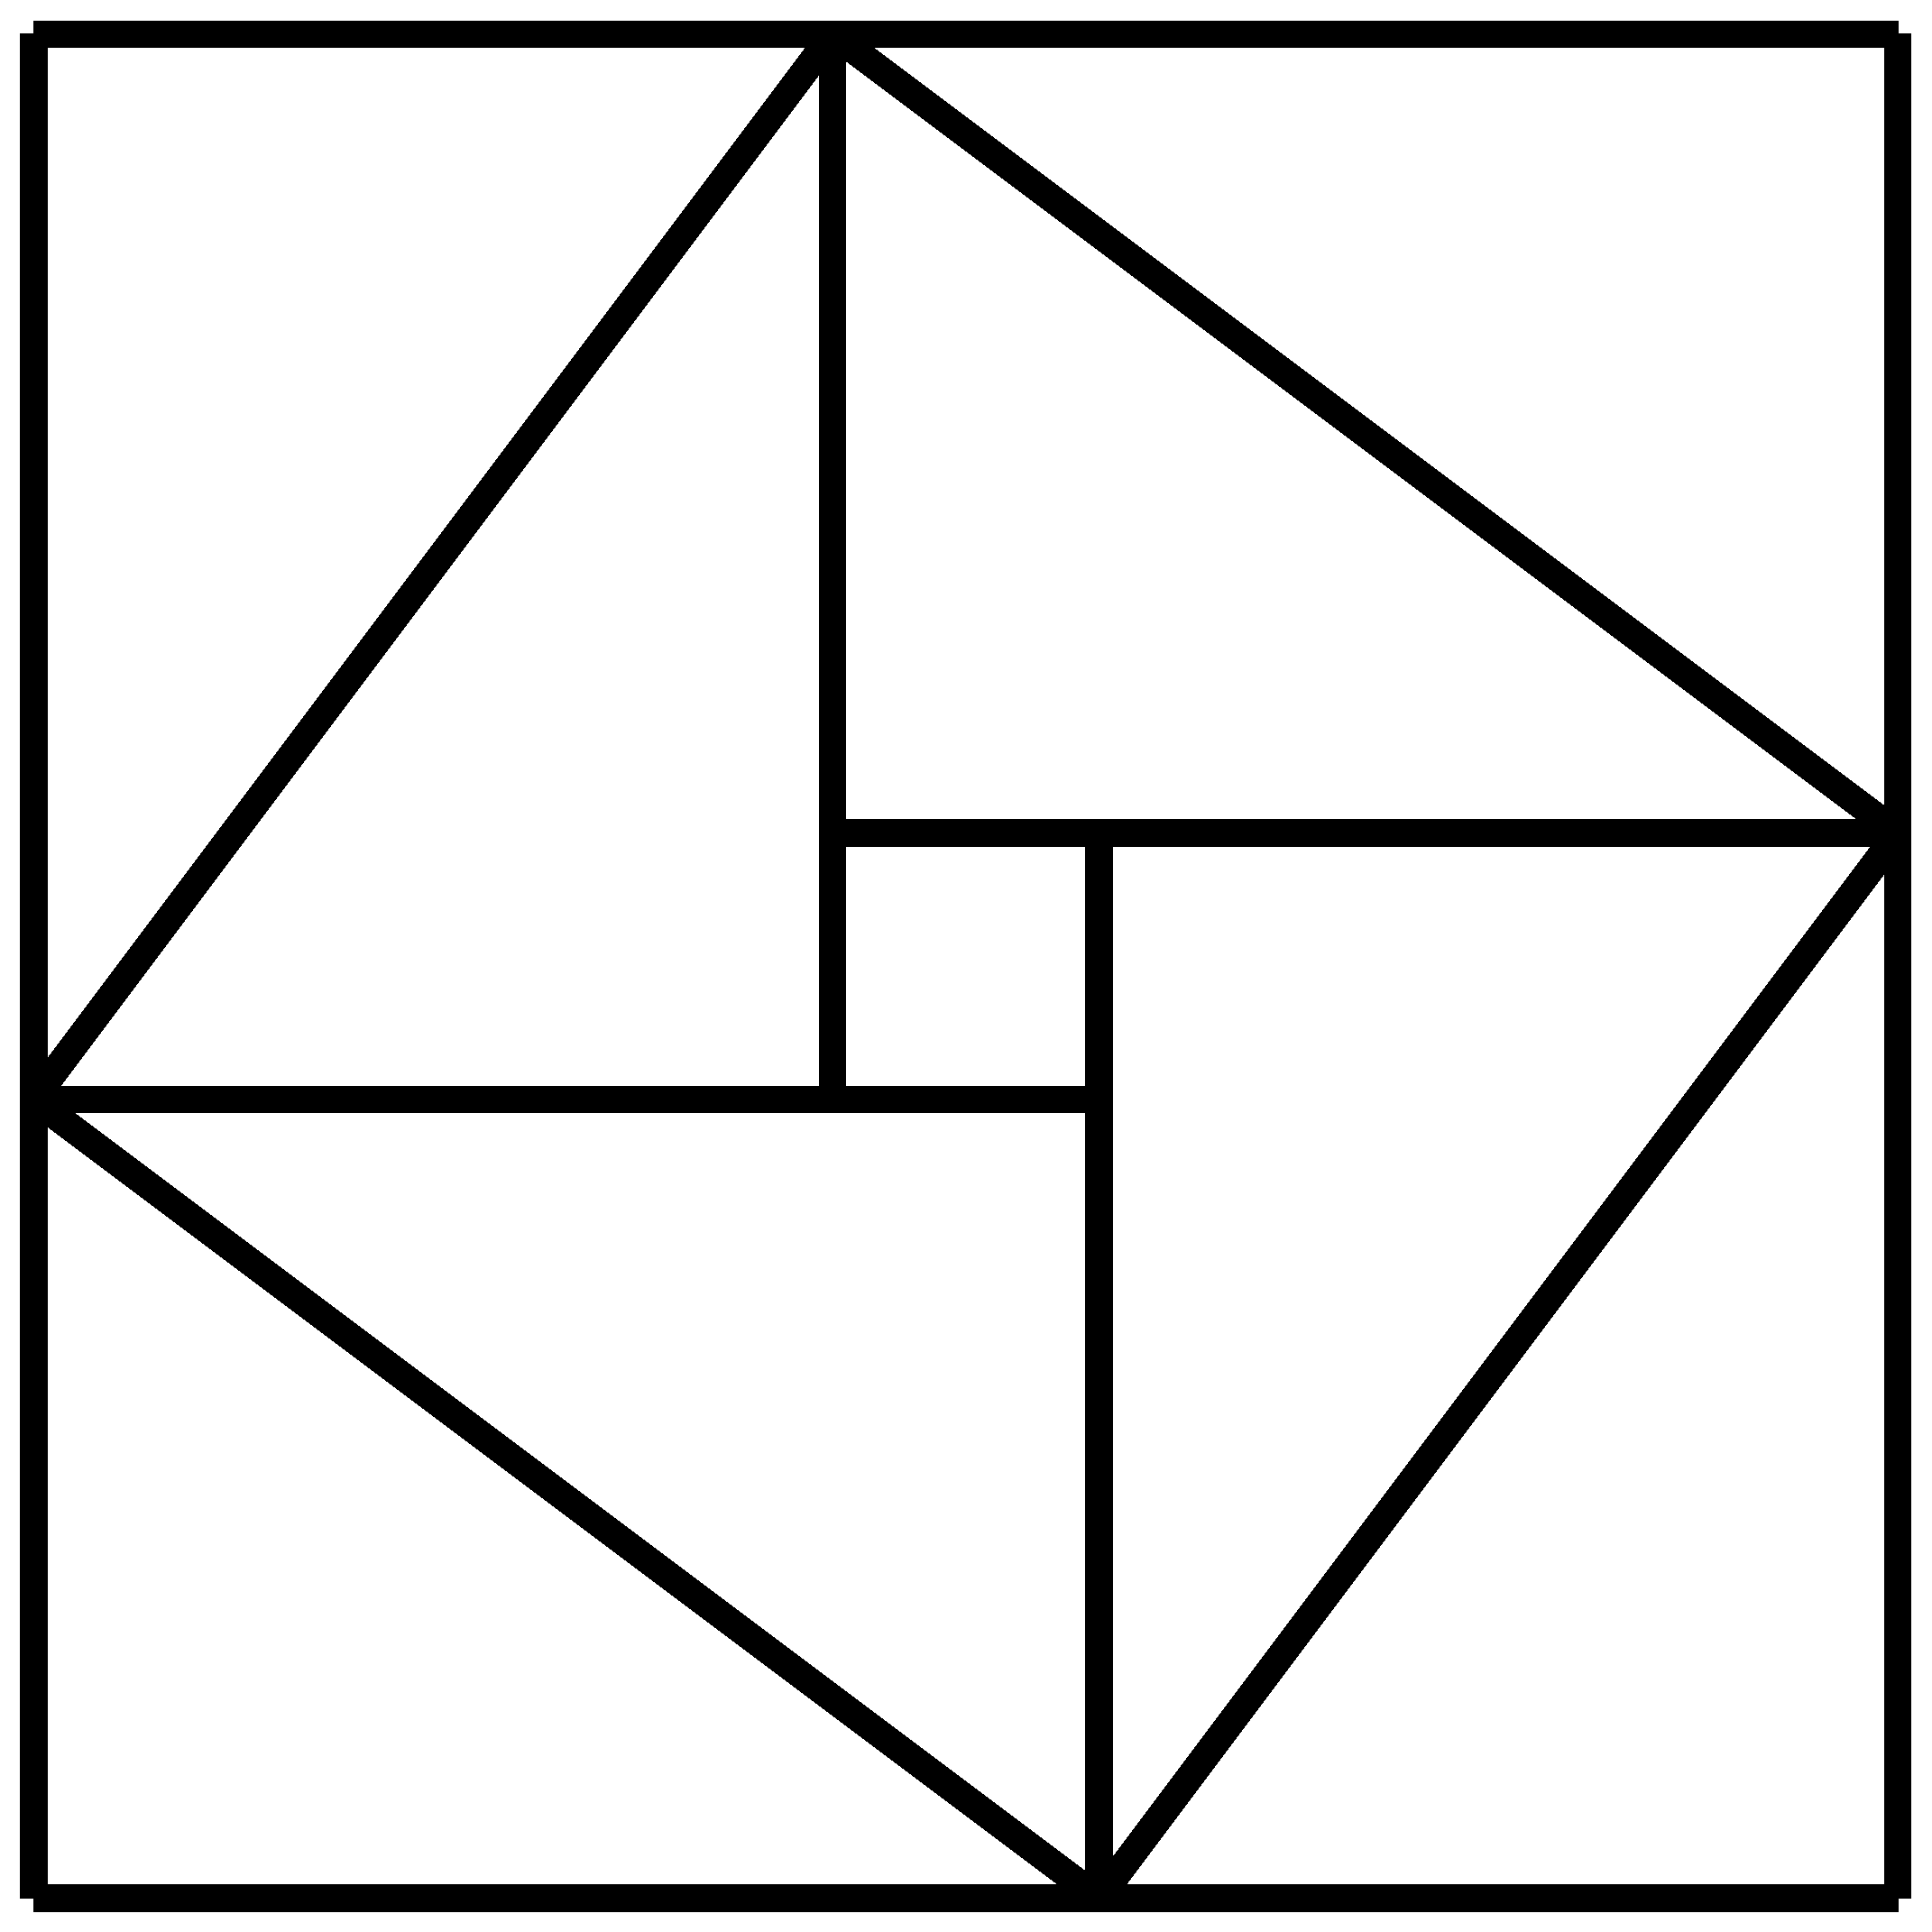
\includegraphics[width=0.2\textwidth]{amss}
  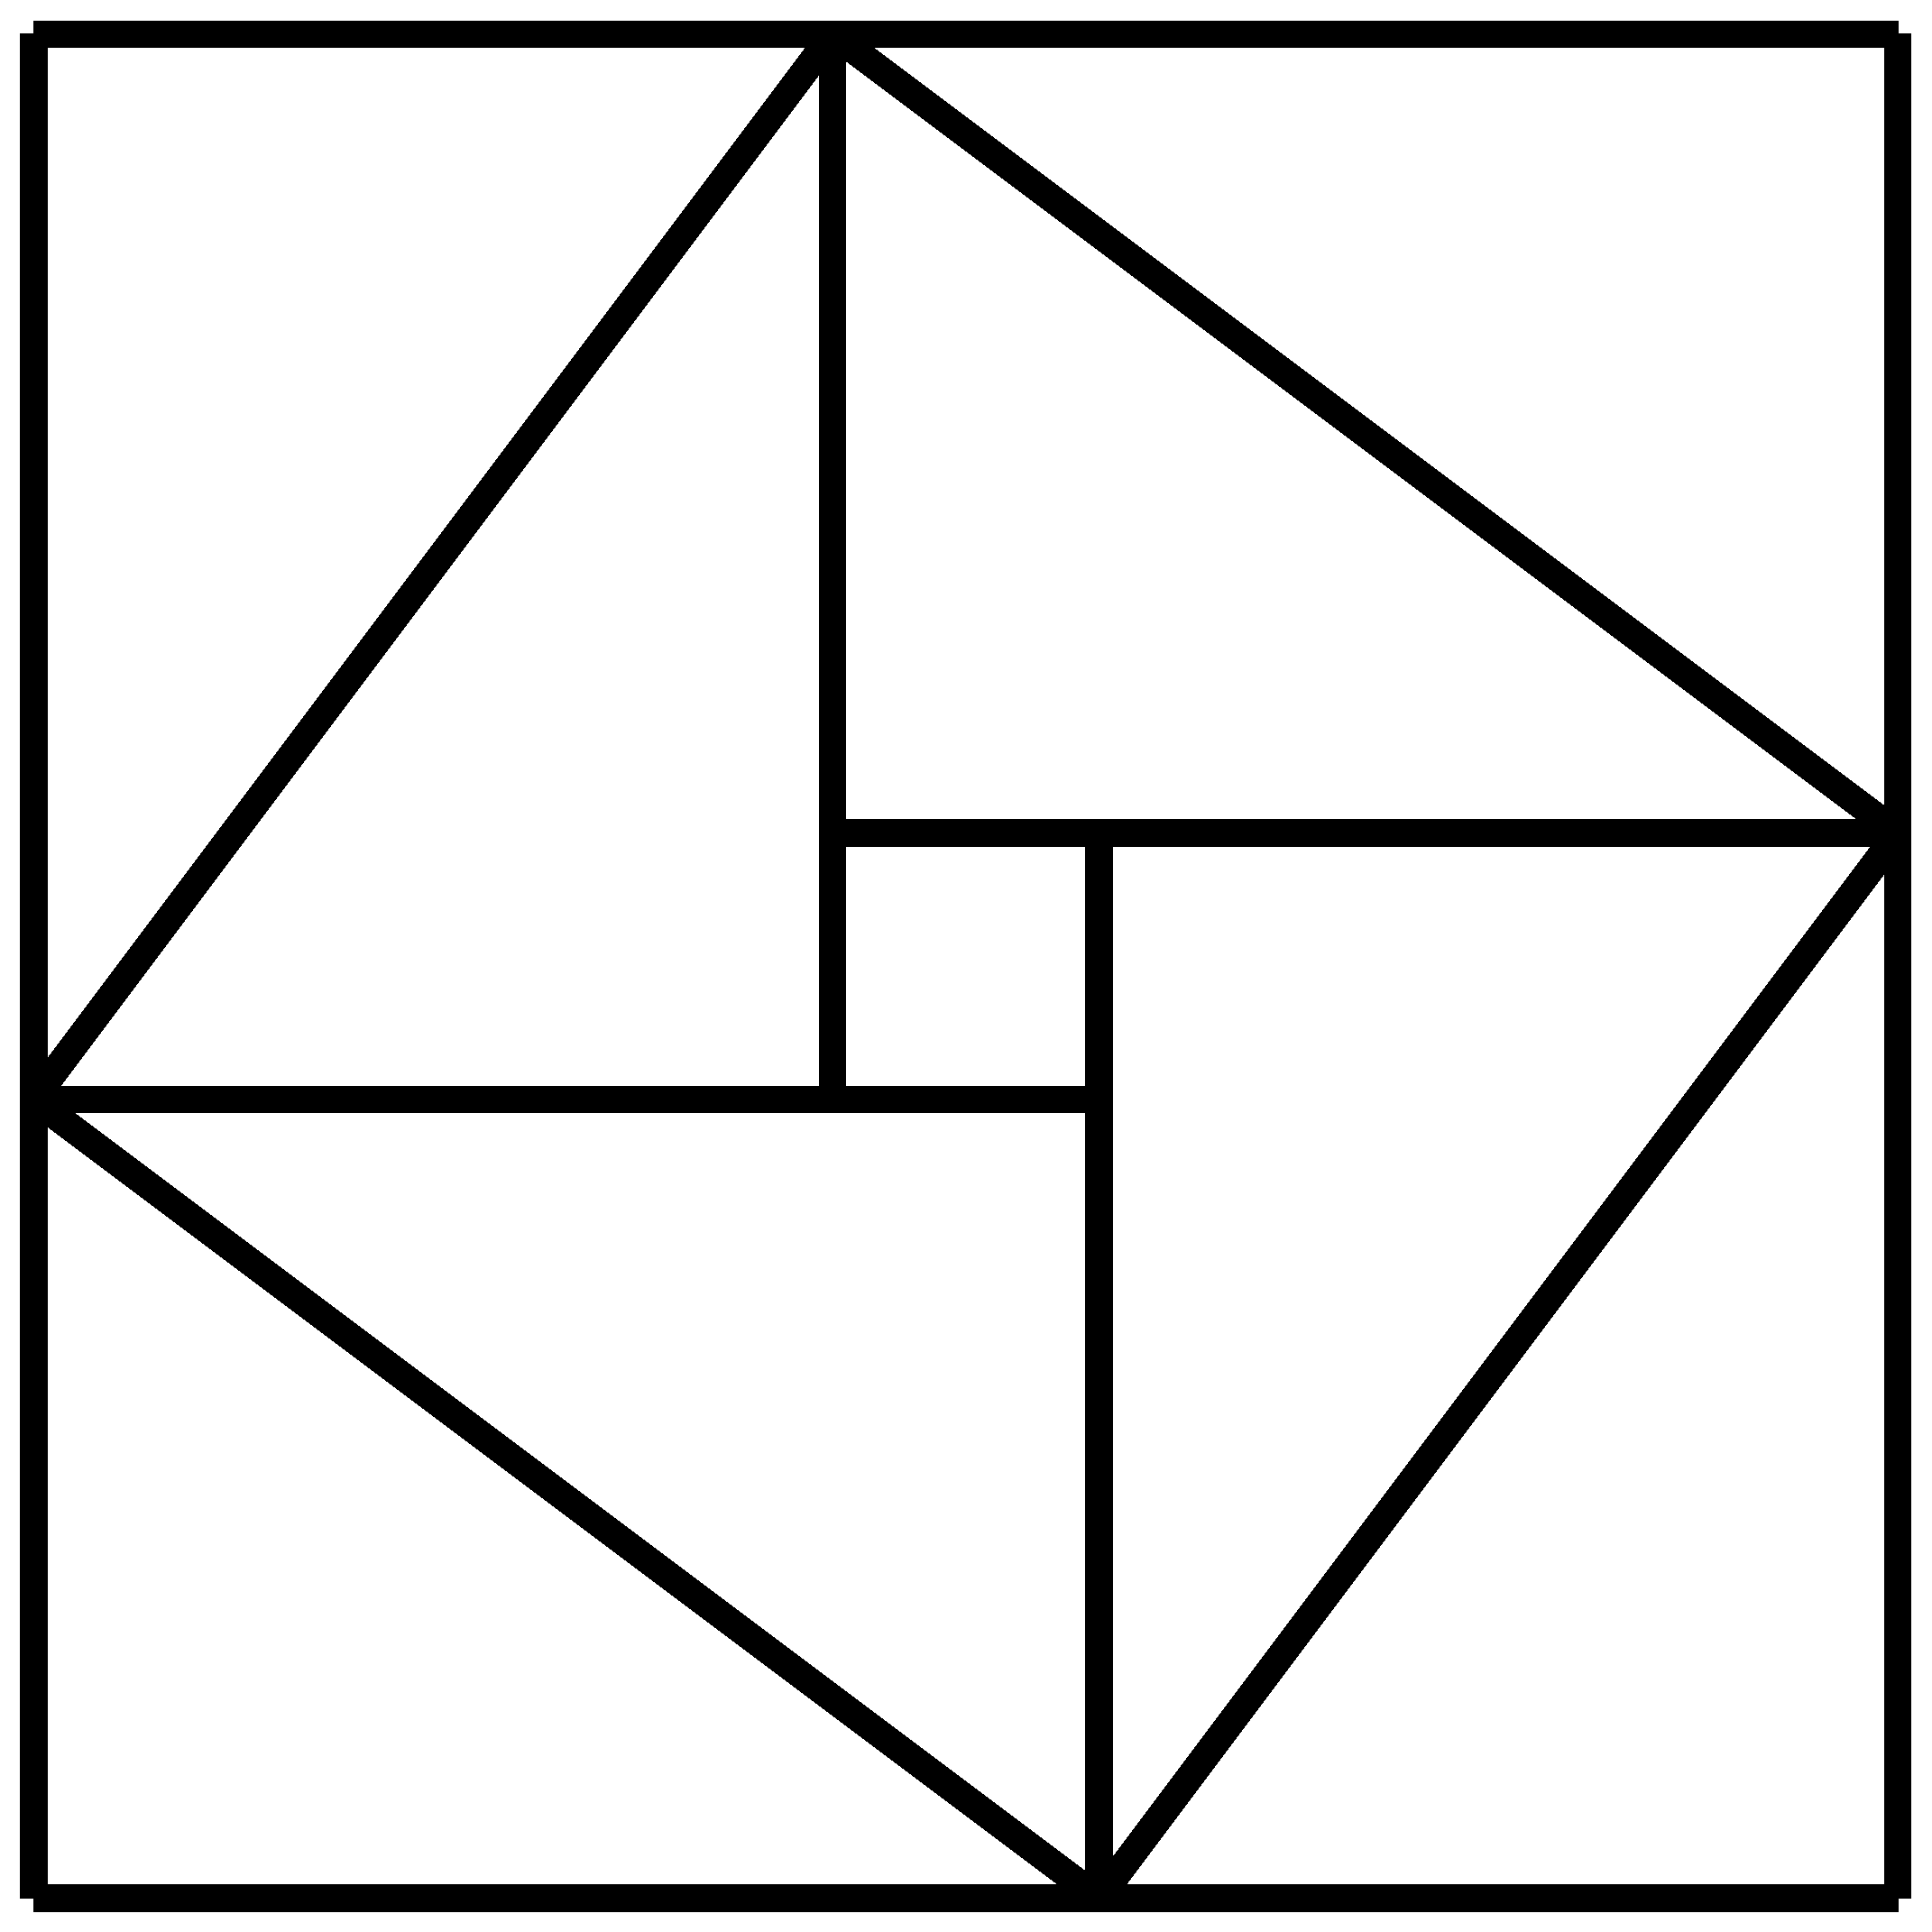
\includegraphics[width=0.2\textwidth]{amss}
 \caption{中科院数学与系统科学研究院院徽(在页面中间)}
 \label{fig:amss1}
\end{figure}

正文正文正文正文正文正文正文正文正文正文正文正文正文。
正文正文正文正文正文正文正文正文正文正文正文正文正文。
正文正文正文正文正文正文正文正文正文正文正文正文正文。
正文正文正文正文正文正文正文正文正文正文正文正文正文。
正文正文正文正文正文正文正文正文正文正文正文正文正文。

\begin{figure}[t]
 \centering
 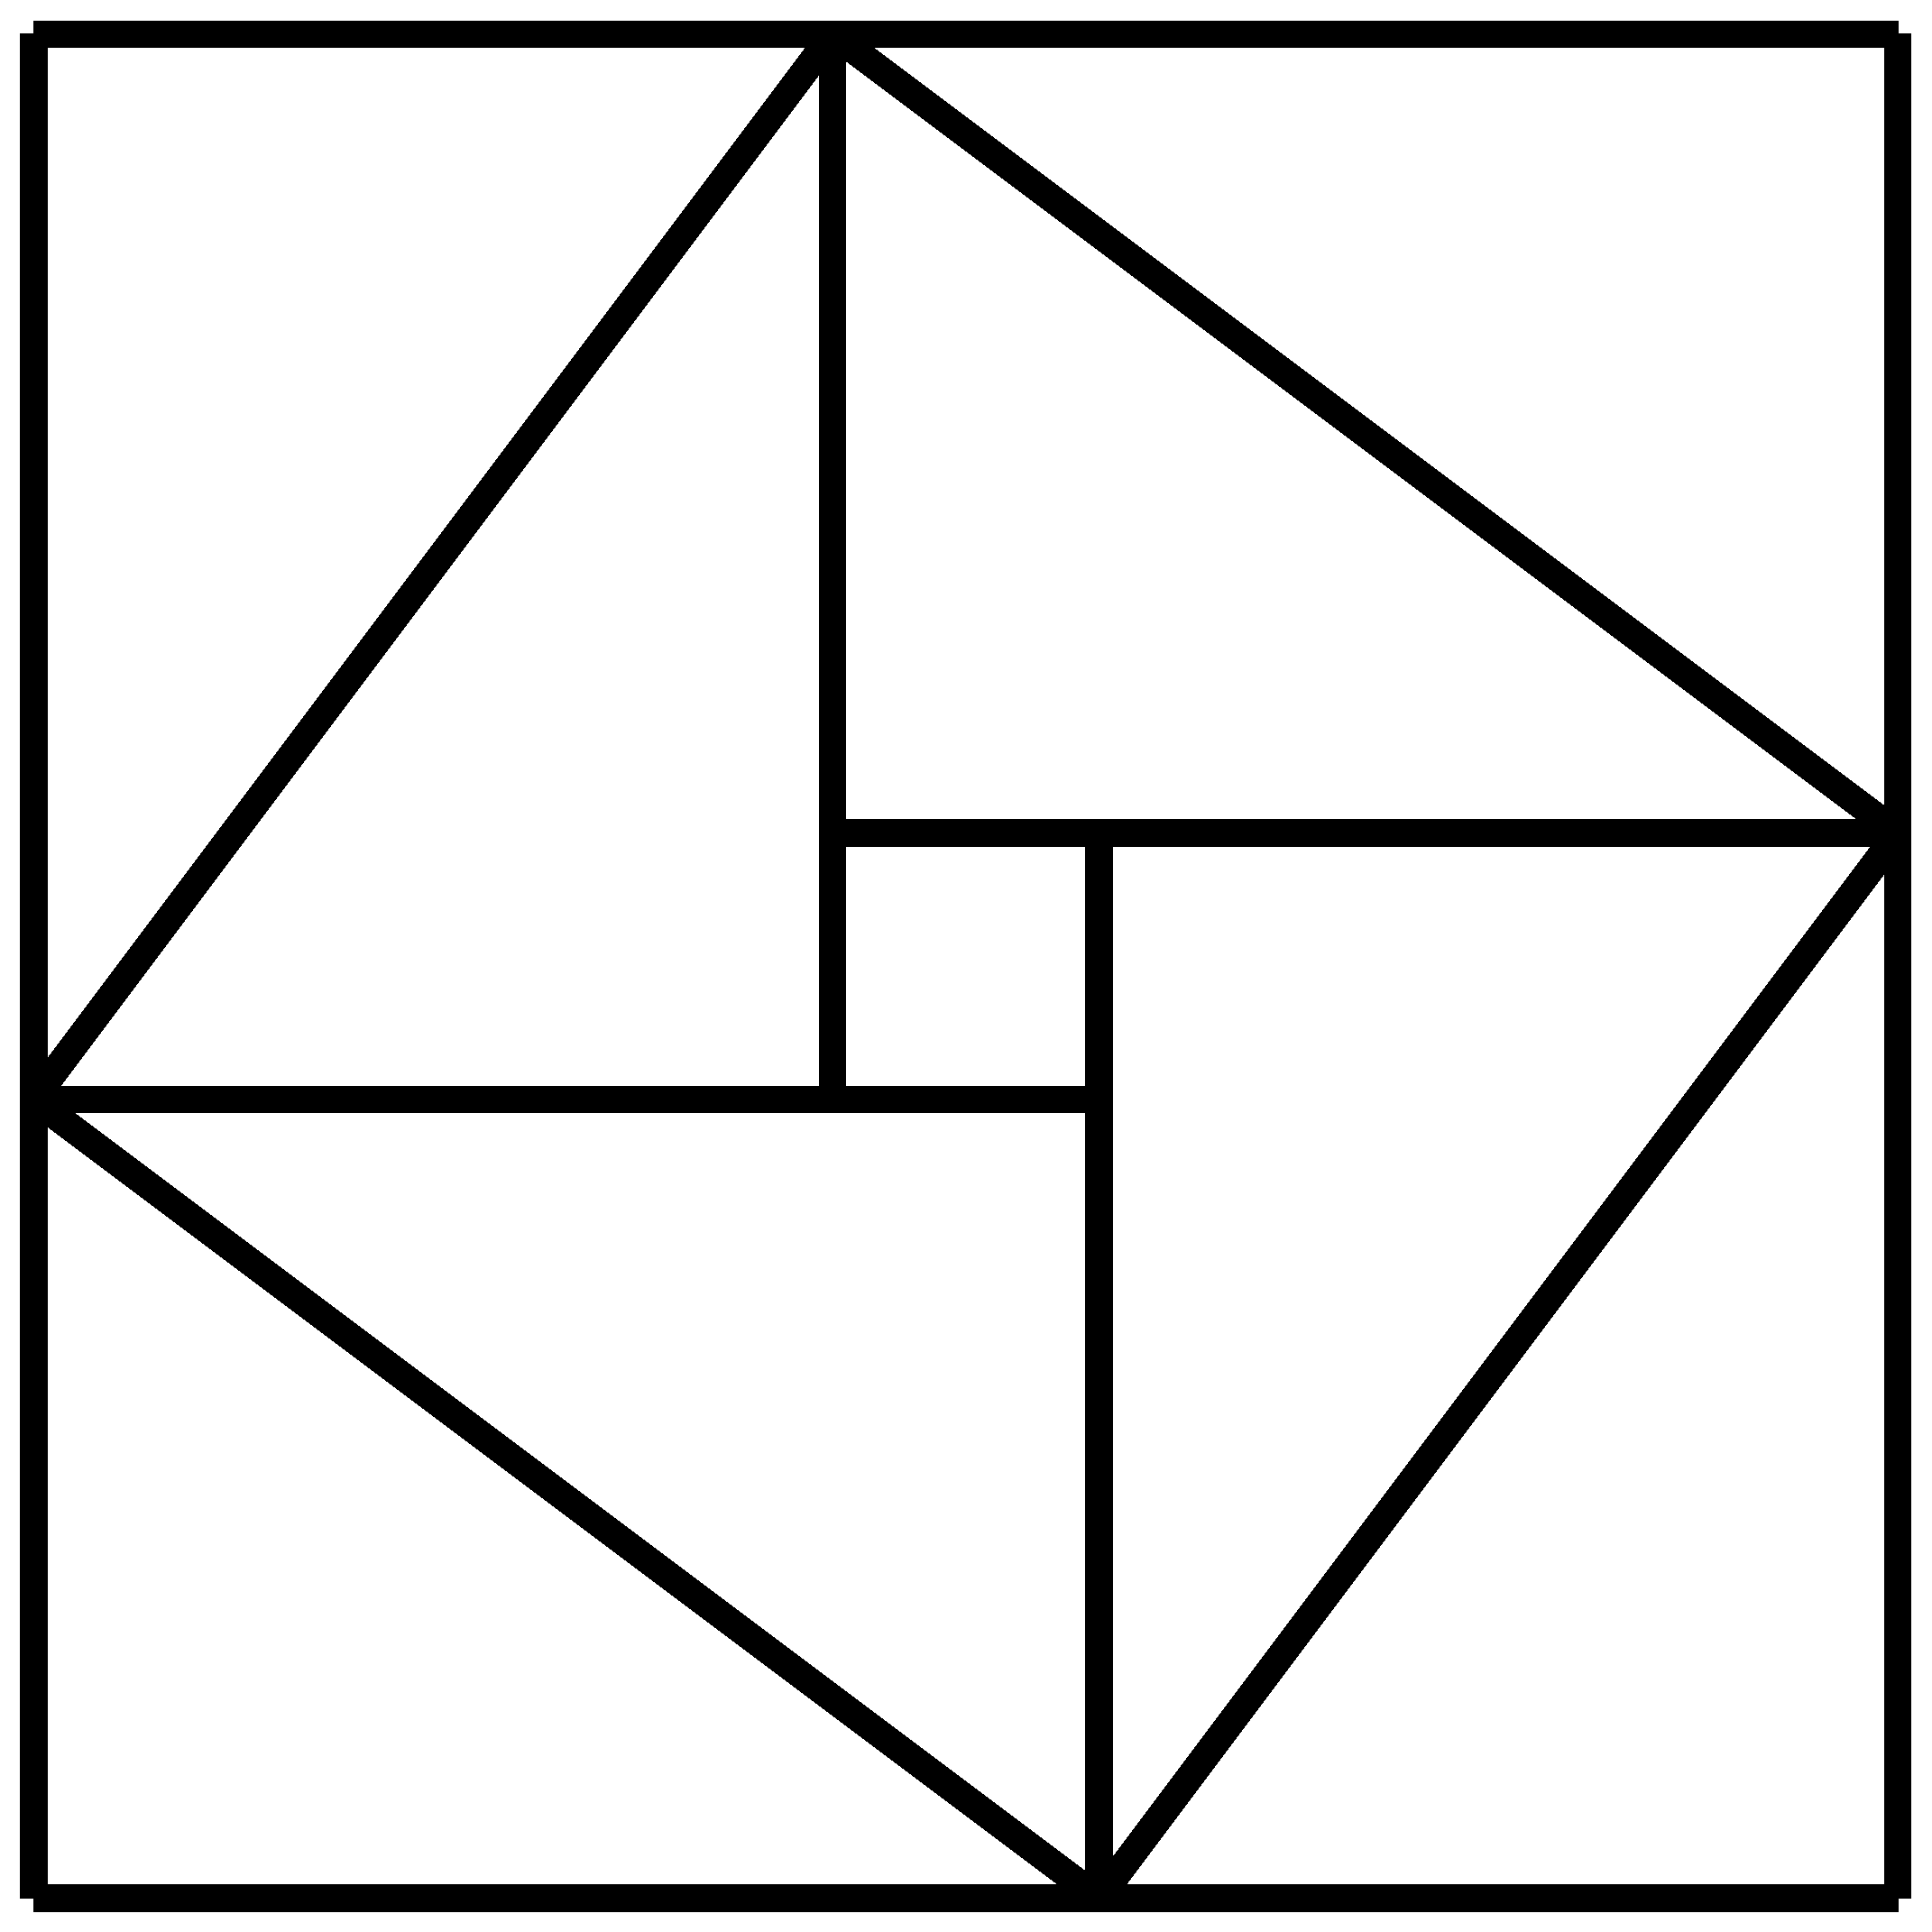
\includegraphics[width=0.2\textwidth]{amss}
 \caption{中科院数学与系统科学研究院院徽(在页面上方)}
 \label{fig:amss2}
\end{figure}

\begin{figure}[t]
 \centering
 \subfloat[]{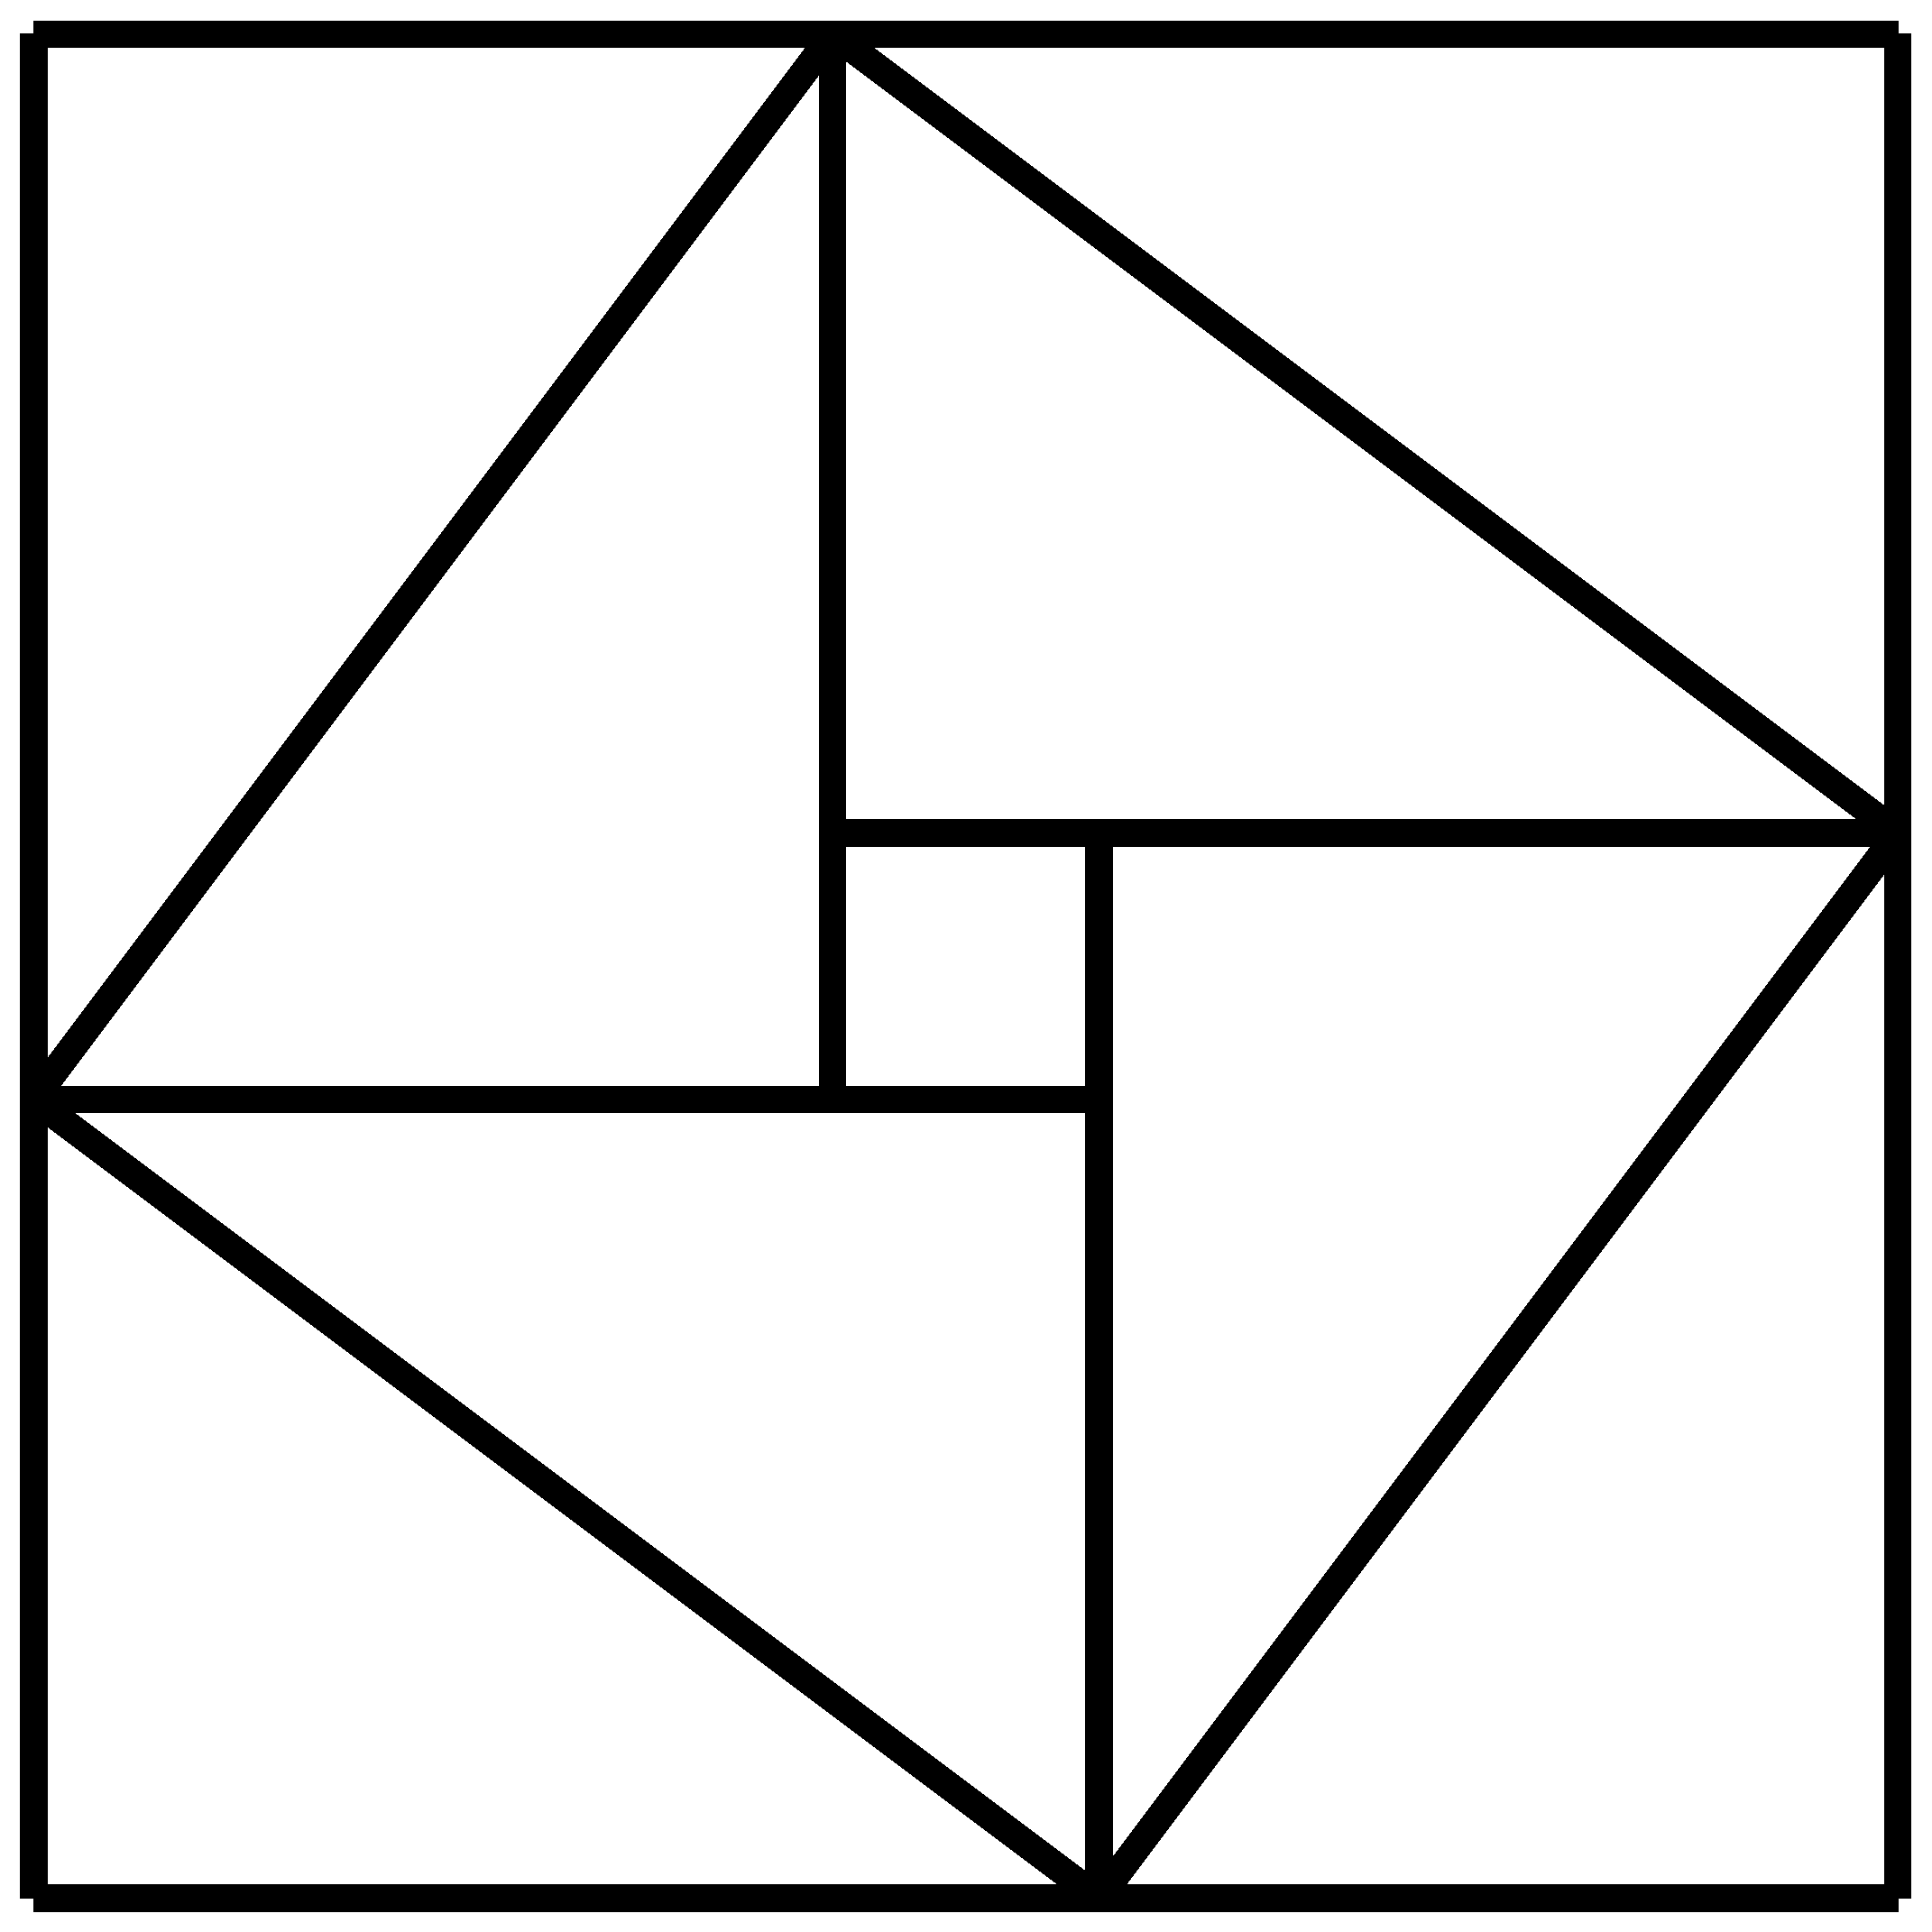
\includegraphics[width=0.2\textwidth]{amss}}
 \subfloat[]{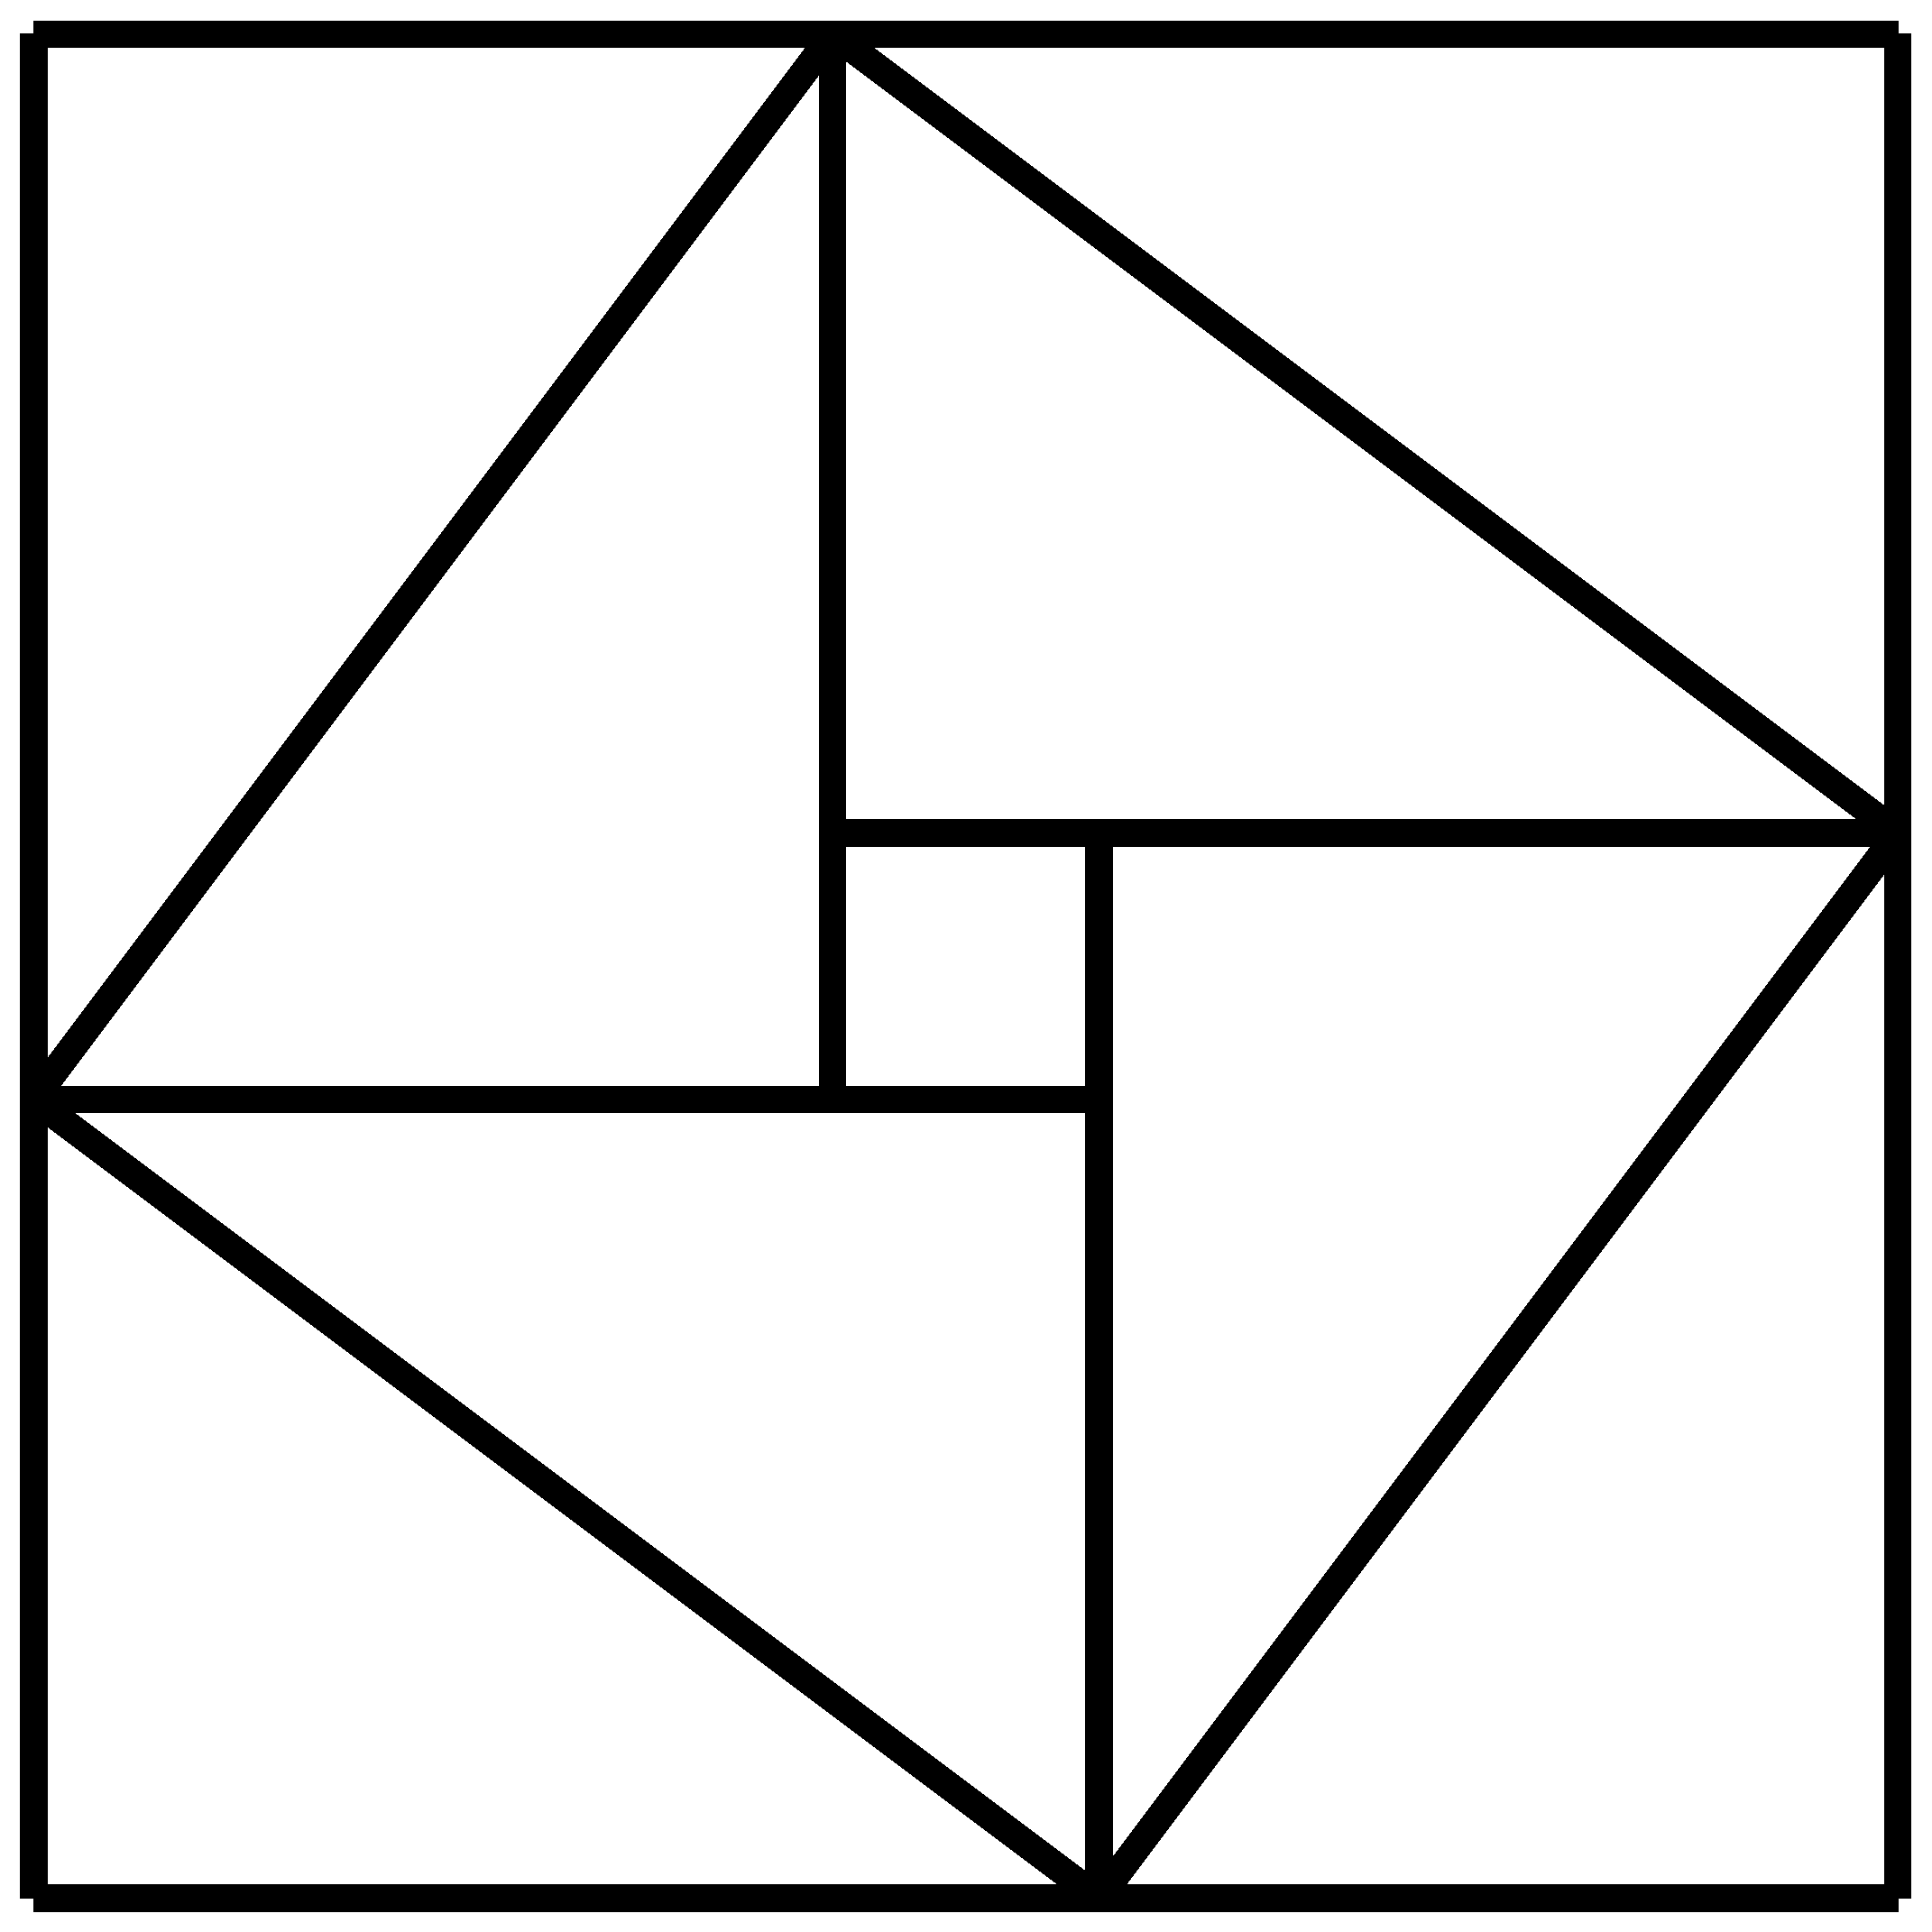
\includegraphics[width=0.2\textwidth]{amss}}
 \caption{中科院数学与系统科学研究院院徽(在页面上方)}
 \label{fig:amss2}
\end{figure}

正文正文正文正文正文正文正文正文正文正文正文正文正文。
正文正文正文正文正文正文正文正文正文正文正文正文正文。
正文正文正文正文正文正文正文正文正文正文正文正文正文。
正文正文正文正文正文正文正文正文正文正文正文正文正文。
正文正文正文正文正文正文正文正文正文正文正文正文正文。

\begin{figure}[b]
 \centering
 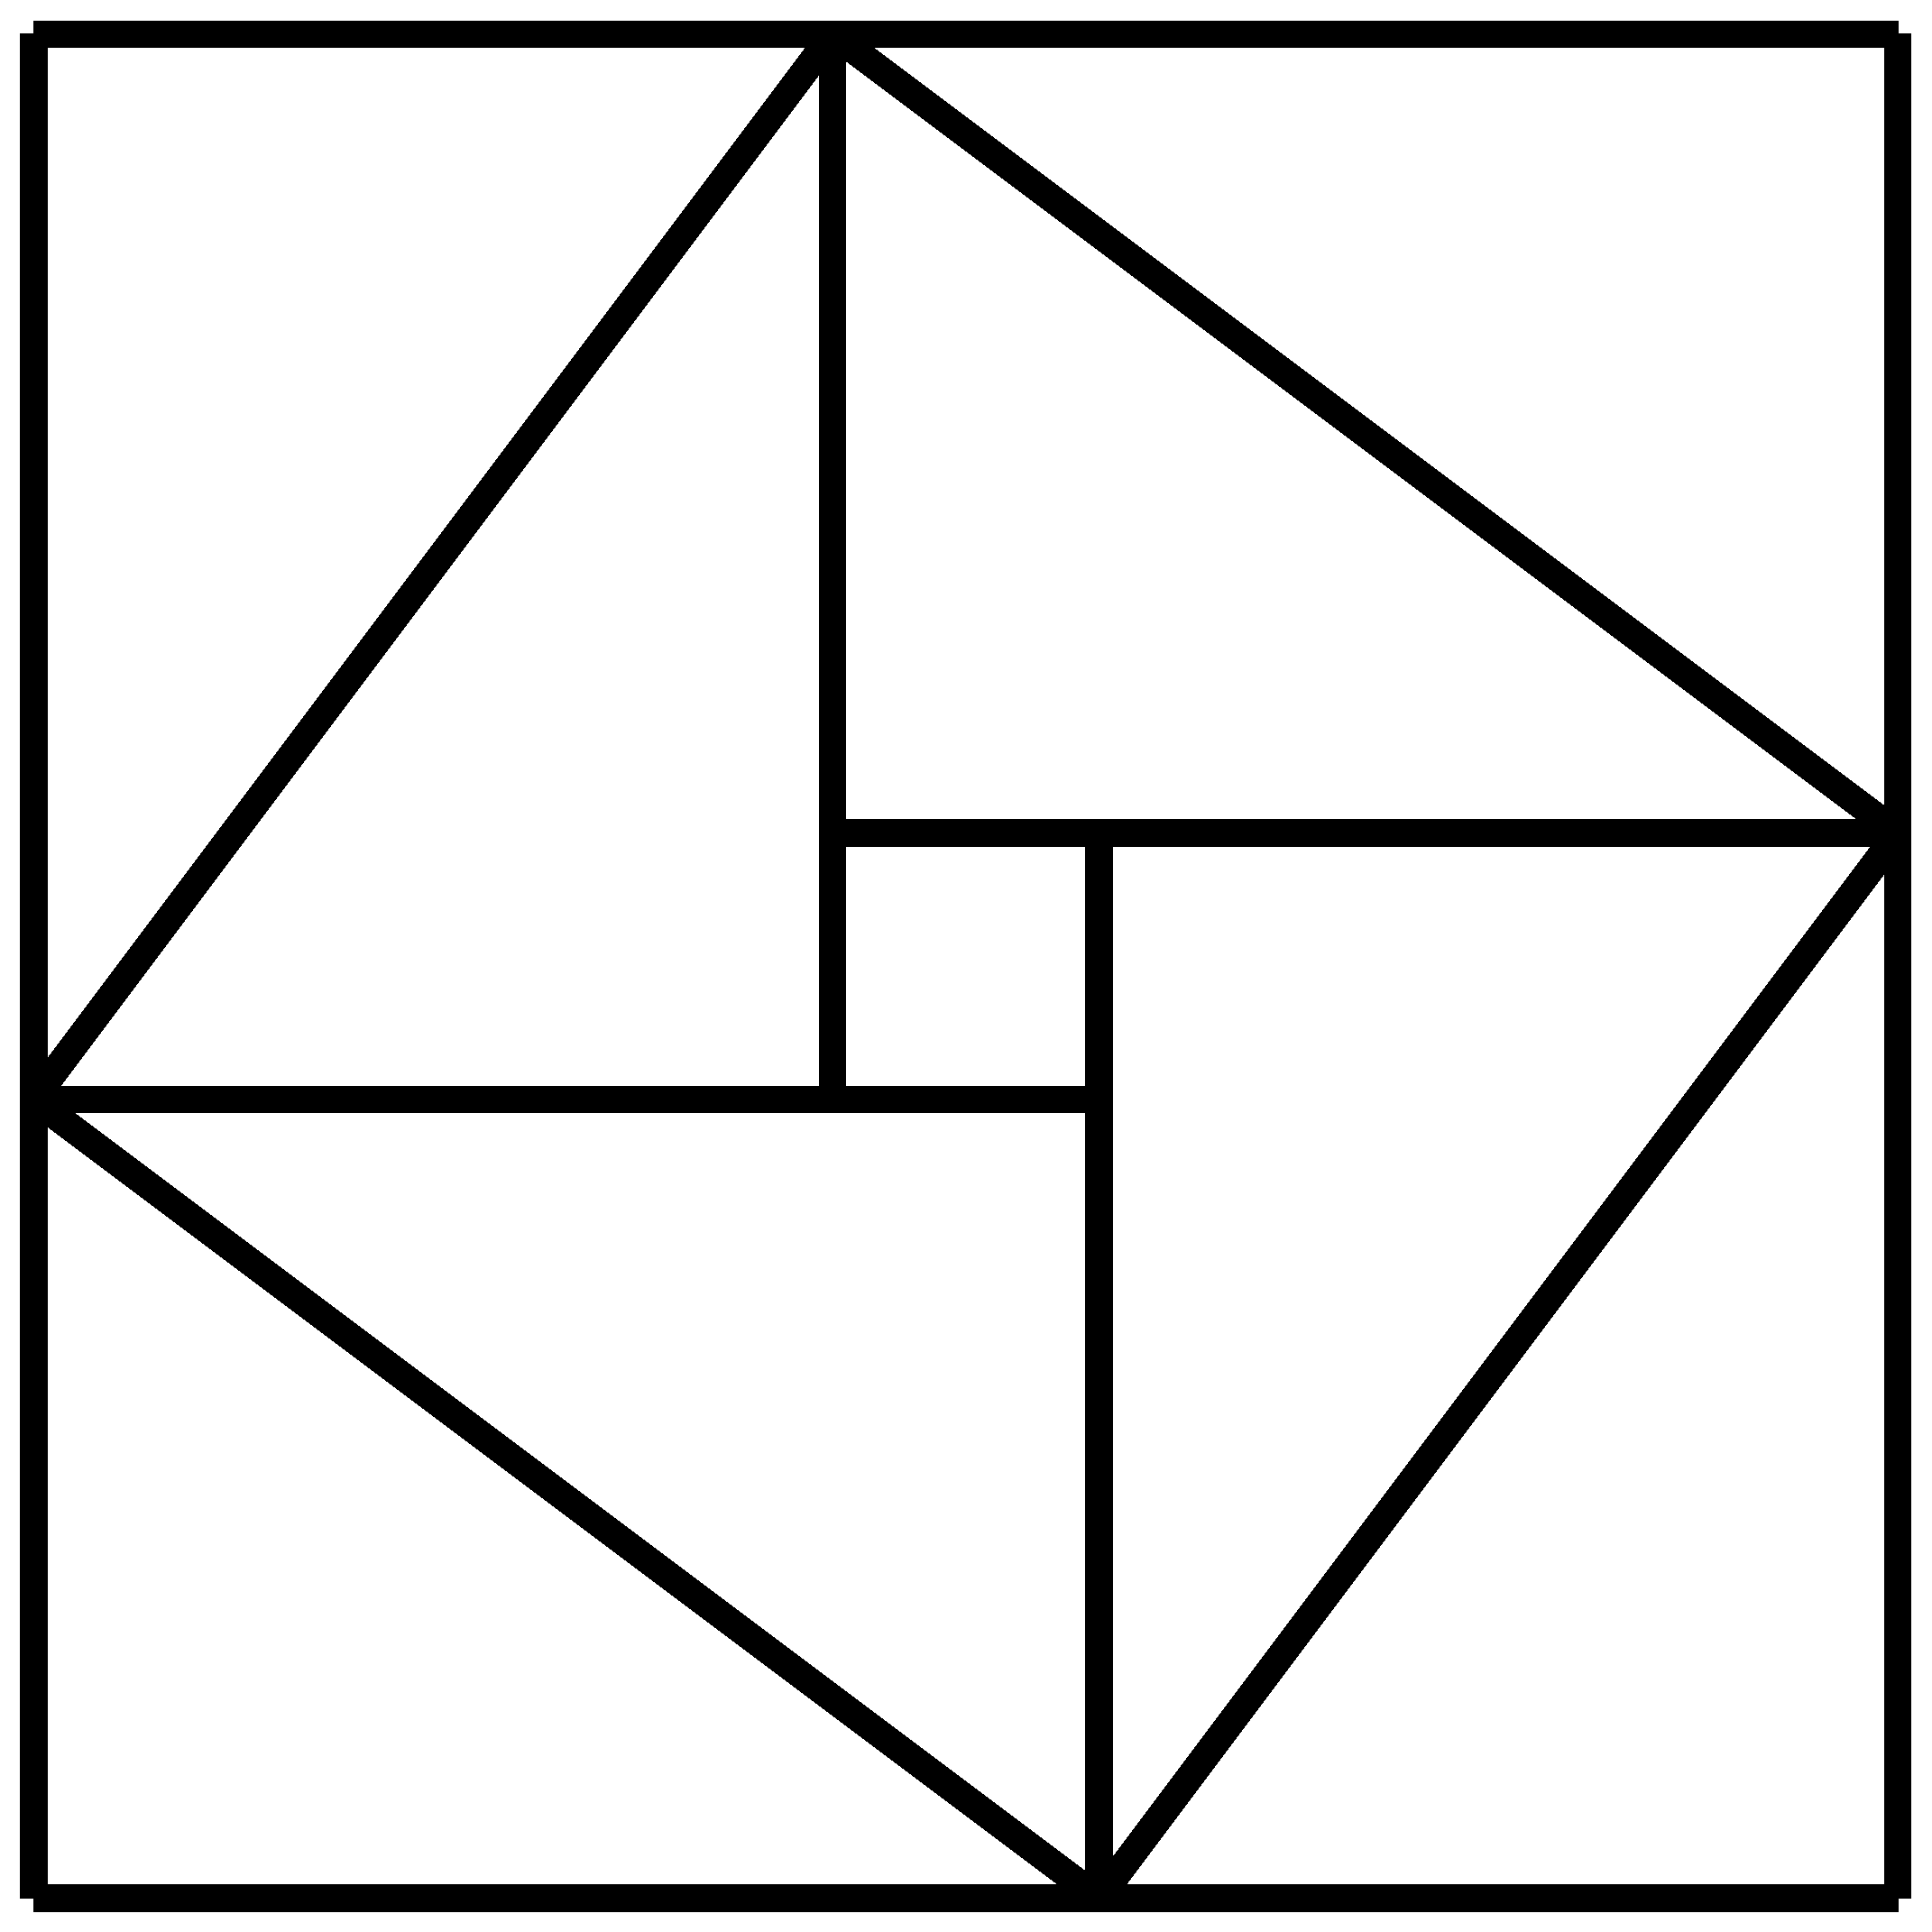
\includegraphics[width=0.2\textwidth]{amss}
 \caption{中科院数学与系统科学研究院院徽(在页面下方)}
 \label{fig:amss3}
\end{figure}


正文正文正文正文正文正文正文正文正文正文正文正文正文。
正文正文正文正文正文正文正文正文正文正文正文正文正文。
正文正文正文正文正文正文正文正文正文正文正文正文正文。
正文正文正文正文正文正文正文正文正文正文正文正文正文。
正文正文正文正文正文正文正文正文正文正文正文正文正文。

正文正文正文正文正文正文正文正文正文正文正文正文正文。
正文正文正文正文正文正文正文正文正文正文正文正文正文。
正文正文正文正文正文正文正文正文正文正文正文正文正文。
正文正文正文正文正文正文正文正文正文正文正文正文正文。
正文正文正文正文正文正文正文正文正文正文正文正文正文。

正文正文正文正文正文正文正文正文正文正文正文正文正文。
正文正文正文正文正文正文正文正文正文正文正文正文正文。
正文正文正文正文正文正文正文正文正文正文正文正文正文。
正文正文正文正文正文正文正文正文正文正文正文正文正文。
正文正文正文正文正文正文正文正文正文正文正文正文正文。
正文正文正文正文正文正文正文正文正文正文正文正文正文。
正文正文正文正文正文正文正文正文正文正文正文正文正文。

正文正文正文正文正文正文正文正文正文正文正文正文正文。
正文正文正文正文正文正文正文正文正文正文正文正文正文。
正文正文正文正文正文正文正文正文正文正文正文正文正文。
正文正文正文正文正文正文正文正文正文正文正文正文正文。
正文正文正文正文正文正文正文正文正文正文正文正文正文。
正文正文正文正文正文正文正文正文正文正文正文正文正文。

正文正文正文正文正文正文正文正文正文正文正文正文正文。
正文正文正文正文正文正文正文正文正文正文正文正文正文。
正文正文正文正文正文正文正文正文正文正文正文正文正文。
正文正文正文正文正文正文正文正文正文正文正文正文正文。
正文正文正文正文正文正文正文正文正文正文正文正文正文。
正文正文正文正文正文正文正文正文正文正文正文正文正文。
正文正文正文正文正文正文正文正文正文正文正文正文正文。

\begin{figure}[p]
 \centering
 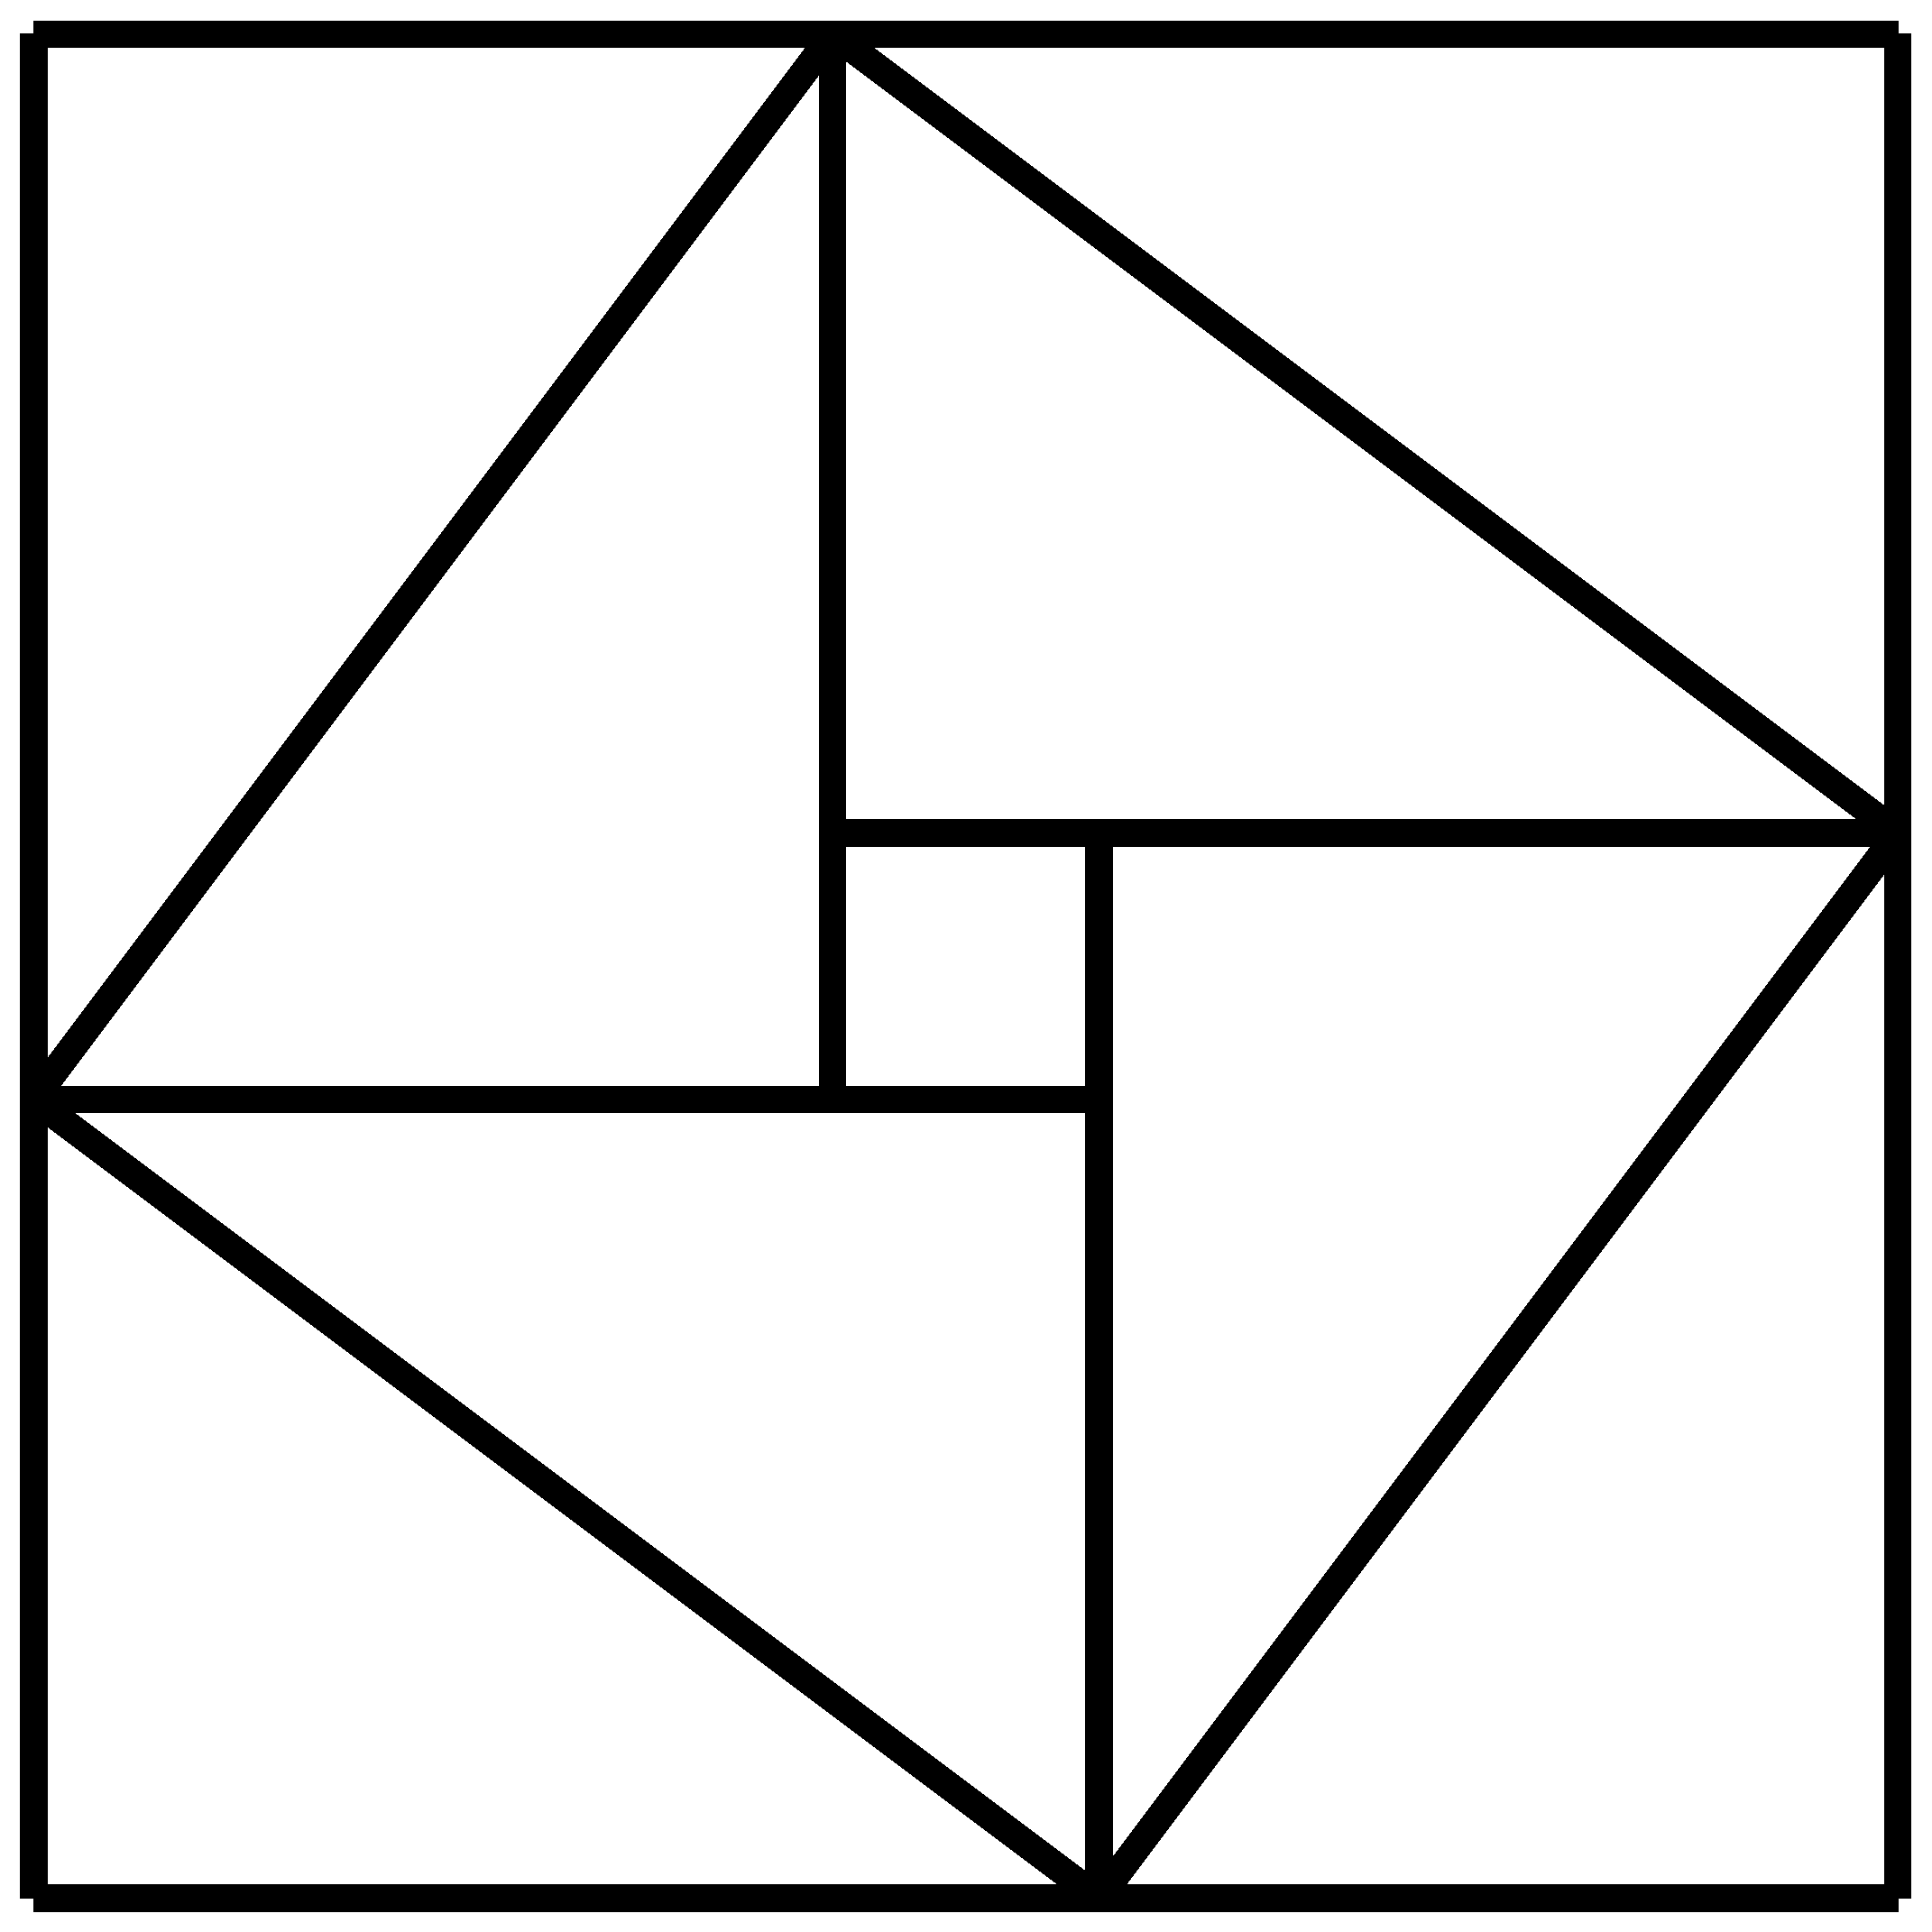
\includegraphics[width=\textwidth]{amss}
 \caption{中科院数学与系统科学研究院院徽(在独立页面中)}
 \label{fig:amss4}
\end{figure}

正文正文正文正文正文正文正文正文正文正文正文正文正文。
正文正文正文正文正文正文正文正文正文正文正文正文正文。
正文正文正文正文正文正文正文正文正文正文正文正文正文。
正文正文正文正文正文正文正文正文正文正文正文正文正文。
正文正文正文正文正文正文正文正文正文正文正文正文正文。
正文正文正文正文正文正文正文正文正文正文正文正文正文。
正文正文正文正文正文正文正文正文正文正文正文正文正文。
正文正文正文正文正文正文正文正文正文正文正文正文正文。
正文正文正文正文正文正文正文正文正文正文正文正文正文。
正文正文正文正文正文正文正文正文正文正文正文正文正文。

  
\chapter{常见问题}
\label{chap:faq}

\newtheoremstyle{question}% name
  {}%      Space above, empty = `usual value'
  {}%      Space below
  {\tt}% Body font
  {}%         Indent amount (empty = no indent, \parindent = para indent)
  {\bfseries}% Thm head font
  {.}%        Punctuation after thm head
  {10pt}% Space after thm head: \newline = linebreak
  {}%         Thm head spec

\newtheoremstyle{answer}% name
  {}%      Space above, empty = `usual value'
  {}%      Space below
  {\rm}% Body font
  {}%         Indent amount (empty = no indent, \parindent = para indent)
  {\bfseries}% Thm head font
  {.}%        Punctuation after thm head
  {10pt}% Space after thm head: \newline = linebreak
  {}%         Thm head spec

\theoremstyle{question}
 \newtheorem{FAQ}{问题~}
\theoremstyle{answer}
 \newtheorem{ANS}{回答~}

\section{表格}

\begin{FAQ}
页眉里论文题目和各章标题中的字母均为大写,不能实现大小写的区别,而我写的论文需要在页眉中出现的标题中区分英文字母的大小写比如:YBaCuO而不是YBACUO。
\end{FAQ}

\begin{ANS}
在 CASthesis.cfg 文件中加上
\begin{verbatim}
\renewcommand\title[2][\CAST@value@title]{%
  \def\CAST@value@title{#2}
  \def\CAST@value@titlemark{#1}}
\def\chaptermark#1{\markboth {{\ifnum \c@secnumdepth>\m@ne
  \if@mainmatter\CTEXthechapter \quad\fi
  \fi #1}}{}}%
\def\sectionmark#1{\markright{{\ifnum \c@secnumdepth >\z@
  \CTEXthesection \quad \fi #1}}}
\end{verbatim}
\end{ANS}


\section{脚注}

\begin{FAQ}
如果在章节标题中加入注脚,则不仅会出现在本章首页的页脚,也会出现在目录的页脚,不知是否能够让其不要出现在目录的页脚中。
\end{FAQ}

\begin{ANS}
可以使用如下的命令来定义章节的标题
\begin{verbatim}
\chapter[出现在目录和页眉的标题]{出现在正文的标题\footnote{这个不会出现在目录中。}}
\end{verbatim}
section、~subsection 等命令也有类似的用法。
\end{ANS}


  % 附录
  \appendix

  
\chapter{中国科学院研究生院学位论文撰写要求}
\label{chap:requires}

学位论文是为申请学位而撰写的学术论文,是评判学位申请者学术水平的主要依据,
也是学位申请者获得学位的必要条件之一。为规范和统一我院研究生学位论文的写作,
根据《中华人民共和国学位条例暂行实施办法》的有关规定,提出以下要求:

\section{基本要求}

学位论文必须是一篇(或由一组论文组成的一篇)系统的、完整的学术论文。
学位论文应是学位申请者本人在导师的指导下独立完成的研究成果,
不得抄袭和剽窃他人成果。学位论文的学术观点必须明确,且逻辑严谨,文字通畅。

\subsection{硕士学位论文}

硕士学位论文要注意在基础学科或应用学科中选择有价值的课题,
对所研究的课题有新的见解,并能表明作者在本门学科上掌握了坚实的基础理论和
系统的专门知识,具有从事科学研究工作或独立担负专门技术工作的能力。

硕士学位论文工作一般在硕士生完成培养计划所规定的课程学习后开始,
应包括文献阅读、开题报告、拟定并实施工作计划、科研调查、实验研究、理论分析
和文字总结等工作环节。硕士学位论文必须有一定的工作量。在论文题目确定后,
用于论文工作的时间一般不得少于一年半。

\subsection{博士学位论文}

博士学位论文要选择在国际上属于学科前沿的课题或对国家经济建设和社会发展
有重要意义的课题,要突出论文在科学和专门技术上的创新性和先进性,
并能表明作者在本门学科上掌握了坚实宽广的基础理论和系统深入的专门知识,
具有独立从事科学研究工作的能力。

博士学位论文工作是培养博士学位研究生最重要的环节,其工作时间一般不应少于两年。
博士研究生入学后,要在导师指导下确定科研方向,收集资料,阅读文献,
进行调查研究,选择研究课题。一般在第二学期,最迟在第三学期通过开题报告
并制定论文工作计划,之后根据论文工作计划分阶段报告科研和论文工作进展情况。

\section{学位论文的组成部分和排列顺序}

学位论文一般由以下几个部分组成:封面、论文摘要、论文目录、正文、参考文献、
发表文章目录、致谢等。

\subsection{封面}

根据原国家标准局《科学技术报告、学位论文和学术论文的编写格式》
(国家标准GB7713-87)的封面要求,特规定中国科学院研究生院研究生学位论文的
封面格式(见样张1和样张2),并提出以下具体要求:

\subsubsection{分类号}

必须在封面左上角注明分类号。一般应注明《中国图书资料分类法》的类号,
同时注明《国际十进分类法UDC》的类号。

\subsubsection{编号}

各培养单位自定。

\subsubsection{密级}

论文必须按国家规定的保密条例在右上角注明密级(如系公开型论文则可不注明密级)。

\subsubsection{论文题目}

学位论文题目应当简明扼要地概括和反映出论文的核心内容,一般不宜超过20个字,
必要时可加副标题。

\subsubsection{指导教师}

指导教师必须是被批准上岗的指导教师。

\subsubsection{申请学位级别}

填硕士学位或博士学位。

\subsubsection{学科、专业名称}

按国家颁布的学科、专业目录中的名称填写。

\subsubsection{论文提交日期和论文答辩日期}

按实际提交和答辩日期填写。

\subsubsection{培养单位}

填写培养单位全称。

\subsubsection{学位授予单位}

填写``中国科学院研究生院''。

\subsection{论文摘要}

论文摘要应概括地反映出本论文的主要内容,主要说明本论文的研究目的、内容、
方法、成果和结论。要突出本论文的创造性成果或新见解,不要与引言相混淆。
中文摘要力求语言精炼准确,字数在500字左右。英文摘要内容要与中文摘要内容一致。
并在英文题目下面第一行写研究生姓名。专业名称用括号括起后,置于姓名之后。
研究生姓名下面的一行写导师姓名,格式为:Directed by......。
无论中英文摘要都必须在摘要页的最下方另起一行,注明本文的关键词(3~5个)。

\subsection{论文目录}

论文目录是论文的提纲,也是论文各章节组成部分的小标题。

\subsection{正文}

正文是学位论文的主体和核心部分,不同学科专业和不同的选题可以有不同的写作方式。
正文一般包括以下几个方面:

\subsubsection{引言}

引言是学位论文主体部分的开端,要求言简意赅,不要与摘要雷同或成为摘要的注解。
除了说明研究目的、方法、结果等外,还应评述国内外研究现状和相关领域中已有的研究成果;
介绍本项研究工作前提和任务,理论依据和实验基础,涉及范围和预期结果以及该论文
在已有的基础上所解决的问题。

\subsubsection{各具体章节}

\subsubsection{结论}

结论是学位论文最终和总体的结论,是整篇论文的归宿。应精炼、准确、完整。
着重阐述作者研究的创造性成果及其在本研究领域中的意义,还可进一步提出
需要讨论的问题和建议。

\subsection{参考文献}

学位论文的撰写应本着严谨求实的科学态度,凡有引用他人成果之处,
均应按论文中所引用的顺序列于文末。参考文献的著录均应符合国家有关标准
(按照GB7714-87 《文后参考文献著录格式》执行)。

1.文献是期刊时,书写格式为: 序号\ 作者. 文章题目. 期刊名,
年份(期数):起止页码

2.文献是图书时,书写格式为: 序号\ 作者. 书名. 版次. 出版地:出版单位,年份.
起止页码

\subsection{发表文章目录}

指学位申请者在学期间在各类正式刊物上发表或已被接受的学术论文。

\subsection{致谢}

表达作者对完成论文和学业提供帮助的老师、同学、领导、同事及亲属的感激之情。

\section{学位论文的书写、装订要求}

(一)中国科学院研究生院研究生学位论文必须用中文书写

1. 论文``题目'':黑体小三号

2. 论文``章'':黑体四号

3. 论文``节'':黑体小四号

4. 正文:宋体小四号

5. 为美观方便起见,要有页眉,奇数页上注明每一章名称,偶数页上注明论文题目。

为了便于国际合作与交流,学位论文亦可有英文或其它文字的副本。

(二)文中的图表、附注、参考文献、公式一律采用阿拉伯数字连续(或分章)编号。
如图1,表1,附注:1,文献(1),公式(1)。图序及图名置于图的下方;
表序及表名置于表的上方;论文中的公式编号用括弧括起来写在右边行末,其间不加虚线。

(三)文中所用单位一律采用国务院发布的《中华人民共和国法定计量单位》,
单位名称和符号的书写方式,应采用国际通用符号。

(四)学位论文封面采用全院统一格式,封面用纸为150克花纹纸,博士学位论文
封面颜色为红色,硕士学位论文封面颜色为蓝色(见样张博士学位论文封面、
硕士学位论文封面)。

(五)学位论文一律用A4打印纸装订。



%%%%%%%%%%%%%%%%%%%%%%%%%%%%%%
%% 附件部分
%%%%%%%%%%%%%%%%%%%%%%%%%%%%%%
\backmatter

  % 参考文献
  % 使用 BibTeX
  \makeatletter % 调节参考文献之间距离
  \renewcommand{\@openbib@code}{\addtolength{\itemsep}{-0.5em}}
  \makeatother
  \bibliography{bib/tex}
  \nocite{*}
  % 不使用 BibTeX
  % 
\begin{thebibliography}{10}

\bibitem{deng:01a}
{邓建松,~彭冉冉,~陈长松}.
\newblock {\em \LaTeXe{}~科技排版指南}.
\newblock 科学出版社,~书号:~7-03-009239-2/TP.1516, 北京, 2001.

\bibitem{wang:00a}
王磊.
\newblock {\em \LaTeXe{}~插图指南}.
\newblock 2000.

\bibitem{zhang:03a}
张林波.
\newblock {\em 关于新版~CCT~的说明}.
\newblock 2003.

\bibitem{lshort-cn}
C\TeX{} 翻译小组.
\newblock {\em lshort~中文版~3.20}.
\newblock 2003.

\bibitem{knuth86e}
Donald~E. Knuth.
\newblock {\em Computer Modern Typefaces}, volume~E of {\em Computers and
  Typesetting}.
\newblock Addison-Wesley, Reading, Massachusetts, 1986.

\bibitem{knuth86d}
Donald~E. Knuth.
\newblock {\em {METAFONT}: The Program}, volume~D of {\em Computers and
  Typesetting}.
\newblock Addison-Wesley, Reading, Massachusetts, 1986.

\bibitem{knuth86c}
Donald~E. Knuth.
\newblock {\em The {METAFONT}book}, volume~C of {\em Computers and
  Typesetting}.
\newblock Addison-Wesley, Reading, Massachusetts, 1986.

\bibitem{knuth86b}
Donald~E. Knuth.
\newblock {\em {TeX}: The Program}, volume~B of {\em Computers and
  Typesetting}.
\newblock Addison-Wesley, Reading, Massachusetts, 1986.

\bibitem{knuth86a}
Donald~E. Knuth.
\newblock {\em The {TeX}book}, volume~A of {\em Computers and Typesetting}.
\newblock Addison-Wesley, Reading, Massachusetts, 1986.

\bibitem{lamport85a}
Leslie Lamport.
\newblock {\em {LaTeX} --- A Document Preparation System: User's Guide and
  Reference Manual}.
\newblock Addison-Wesley, Reading, Massachusetts, 2nd edition, 1985.

\end{thebibliography}


  % 发表文章目录
  
\begin{publications}{99}

\item Ji-Hong Zhang, Ling-Yun Wu and Xiang-Sun Zhang.
  Reconstruction of DNA sequencing by hybridization.
  Bioinformatics (SCI), vol 19(1), pages 14-21, 2003.

\item 吴凌云.
  C\TeX{} FAQ (常见问题集).
  2004.

\end{publications}


  % 个人简历
  
\begin{resume}

\begin{resumesection}{基本情况}
吴凌云,男,福建省屏南县人,1975 年~11 月出生,未婚,
中国科学院数学与系统科学研究院在读博士研究生。
\end{resumesection}

\begin{resumelist}{教育状况}
1993 年~9 月至~1997 年~7 月,武汉大学数学系,本科,专业:应用数学。

1997 年~9 月至~2002 年~7 月,中国科学院数学与系统科学研究院,
硕博连读研究生,专业:运筹学与控制论。
\end{resumelist}

\begin{resumelist}{工作经历}
无。
\end{resumelist}

\begin{resumelist}{研究兴趣}
运筹学及其应用,人工神经网络,组合优化,生物信息学。
\end{resumelist}

\begin{resumelist}{联系方式}
通讯地址:北京市~2734 信箱,中科院数学与系统科学研究院应用数学所

邮编:100080

E-mail: aloft@ctex.org
\end{resumelist}

\end{resume}


  % 致谢
  
\begin{thanks}

值此论文完成之际,谨在此向多年来给予我关心和帮助的老师、同学、
朋友和家人表示衷心的感谢!

......

\vskip 18pt

谨把本文献给我最敬爱的父亲!

\end{thanks}



\end{document}
